\chapter{Polynomien kertolasku}

\subsection*{Polynomin kertominen monomilla}

Polynomeja voi kertoa keskenään aivan kuten reaalilukuja. Yksinkertaisin tapaus on polynomin kertominen monomilla.

\subsubsection*{Esimerkkejä}
\begin{itemize}
    \item $2x(3x^2+5x+7) = 6x^3+10x^2+14x$
    \item $5x(3y^2+4y) = 15xy^2+20xy$
    \item $x(y+z) = xy+xz$
\end{itemize}

\subsection*{Kahden binomin tulo}

Toinen yksinkertainen tapaus on kahden binomin tulo. Tällöin kerrotaan termeittäin ja summataan.

\subsubsection*{Esimerkkejä}
\begin{itemize}
    \item $(x+y)(z+w) = xz+xw+yz+yw$
    \item $(ax+by)(x+y) = ax^2+axy+bxy+by^2 = ax^2+(a+b)xy+by^2$
    \item $(x-5)(x-7) = x^2-7x-5x+35 = x^2-12x+35$
\end{itemize}

\subsection*{Yleinen kertolasku}

Osittelulain nojalla kahden polynomin tulo saadaan laskemalla yhteen kaikki
termit, jotka saadaan kertomalla termi ensimmäisestä ja toinen termi toisesta
polynomista.

\newcommand{\pbezier}[4]{
	\pgfmathsetmacro{\PBxa}{#1}
	\pgfmathsetmacro{\PBxb}{#2}
	\pgfmathsetmacro{\PBya}{#3}
	\pgfmathsetmacro{\PByb}{#3+#4}
	\pgfmathsetmacro{\PBca}{0.8 * \PBxa + 0.2 * \PBxb}
	\pgfmathsetmacro{\PBcb}{0.2 * \PBxa + 0.8 * \PBxb}
	\draw[color=red] (\PBxa, \PBya) .. controls (\PBca, \PByb) and (\PBcb, \PByb) .. (\PBxb, \PBya);
}

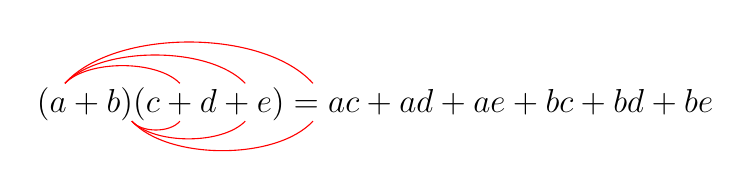
\begin{tikzpicture}
\draw node[right] {\large $(a+b)(c+d+e) = ac+ad+ae+bc+bd+be$};

\pgfmathsetmacro{\klAx}{0.48}
\pgfmathsetmacro{\klBx}{1.33}
\pgfmathsetmacro{\klCx}{1.94}
\pgfmathsetmacro{\klDx}{2.77}
\pgfmathsetmacro{\klEx}{3.63}
\pgfmathsetmacro{\klLo}{-0.22}
\pgfmathsetmacro{\klHi}{0.26}

\pbezier{\klAx}{\klCx}{\klHi}{0.3}
\pbezier{\klAx}{\klDx}{\klHi}{0.48}
\pbezier{\klAx}{\klEx}{\klHi}{0.7}

\pbezier{\klBx}{\klCx}{\klLo}{-0.15}
\pbezier{\klBx}{\klDx}{\klLo}{-0.3}
\pbezier{\klBx}{\klEx}{\klLo}{-0.5}
\end{tikzpicture}

Esimerkiksi polynomien $x-3$ ja $x^2-4x+3$ tulo voidaan laskea vastaavasti:

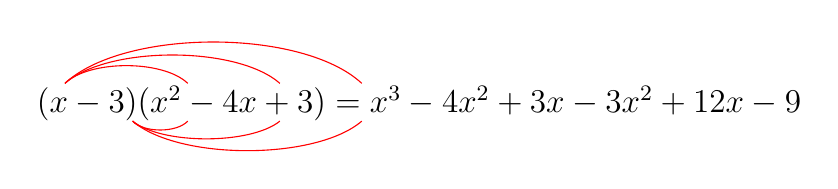
\begin{tikzpicture}
\draw node[right] {\large $(x-3)(x^2-4x+3) = x^3-4x^2+3x-3x^2+12x-9$};

\pgfmathsetmacro{\klAx}{0.48}
\pgfmathsetmacro{\klBx}{1.34}
\pgfmathsetmacro{\klCx}{2.04}
\pgfmathsetmacro{\klDx}{3.21}
\pgfmathsetmacro{\klEx}{4.25}
\pgfmathsetmacro{\klLo}{-0.22}
\pgfmathsetmacro{\klHi}{0.26}

\pbezier{\klAx}{\klCx}{\klHi}{0.3}
\pbezier{\klAx}{\klDx}{\klHi}{0.48}
\pbezier{\klAx}{\klEx}{\klHi}{0.7}

\pbezier{\klBx}{\klCx}{\klLo}{-0.15}
\pbezier{\klBx}{\klDx}{\klLo}{-0.3}
\pbezier{\klBx}{\klEx}{\klLo}{-0.5}
\end{tikzpicture}


Sievennetyksi vastaukseksi saadaan siis $x^3-7x^2+15x-9$.

\begin{esimerkki}
\begin{align*}
&\hspace{0.5cm}(x^4-3x^3+3)(x^3-2x^2+1) \\
&= x^4 (x^3-2x^2+1) - 3x^3 (x^3-2x^2+1) + 3 (x^3-2x^2+1) \\
&= x^4\cdot x^3 + x^4\cdot (-2x^2)+x^4\cdot 1-3x^3\cdot x^3-3x^3(-2x^2)-3x^3\cdot1+3x^3+3(-2x^2)+3\cdot 1 \\
&= x^7-2x^6+x^4-3x^6+6x^5-3x^3+3x^3-6x^2+3 \\
&= x^7-5x^6+6x^5+x^4-6x^2+3
\end{align*}
\end{esimerkki}

\section{Muistikaavat}

Eräitä polynomien kertolaskuja tarvitaan niin usein, että niitä kutsutaan muistikaavoiksi.

\laatikko{
    Muistikaavat
    \begin{itemize}
        \item $(a+b)^2 = a^2+2ab+b^2$
        \item $(a-b)^2 = a^2-2ab+b^2$
        \item $(a+b)(a-b) = a^2-b^2$
    \end{itemize}
}

Nämä kaavat voidaan helposti todistaa laskemalla.

\subsubsection*{Summan neliö}

\begin{align*}
(a+b)^2 &= (a+b)(a+b) &\emph{neliön määritelmä} \\
&= a(a+b)+b(a+b) &\emph{osittelulaki} \\
&= a^2+ab+ba+b^2 &\emph{osittelulaki} \\
&= a^2+ab+ab+b^2 &\emph{reaaliluvuille $ba=ab$} \\
&= a^2+2ab+b^2
\end{align*}

\subsubsection*{Erotuksen neliö}

\begin{align*}
(a-b)^2 &= (a-b)(a-b) &\emph{neliön määritelmä} \\
&= a(a-b)-b(a-b) &\emph{osittelulaki} \\
&= a^2-ab-ba+b^2 &\emph{osittelulaki} \\
&= a^2-ab-ab+b^2 &\emph{reaaliluvuille $ba=ab$} \\
&= a^2-2ab+b^2
\end{align*}

\subsubsection*{Summan ja erotuksen tulo}

\begin{align*}
(a+b)(a-b) &= a(a-b)+b(a-b) &\emph{osittelulaki} \\
&= a^2-ab+ba-b^2 &\emph{osittelulaki} \\
&= a^2-ab+ab-b^2 &\emph{reaaliluvuille $ba=ab$} \\
&= a^2-b^2
\end{align*}

\laatikko{
    Esimerkkejä
    \begin{itemize}
        \item $(3x+2y)^2 = (3x+2y)(3x+2y) = 9x^2+2\cdot 3x\cdot 2y+4y^2 = 9x^2+12xy+4y^2$
        \item $995^2 = (1000-5)^2 = 1000^2-2\cdot 1000\cdot 5+5^2 = 1000000-10000+25 = 990025$
        \item $104\cdot 96 = (100+4)(100-4) = 100^2 - 4^2 = 10000 - 16 = 9984$
    \end{itemize}
    }

\section{Tekijöihinjako}

Matematiikan 1. kurssilla on käsitelty lukujen jakamista tekijöihin.
Esimerkiksi luvun $12$ {\bf tekijät} ovat $1$, $2$, $3$, $4$, $6$ ja $12$. Nämä ovat sellaisia
lukuja, joista saadaan $12$ kertomalla ne jollain kokonaisluvulla. Sanotaan myös, että luvun $12$
{\bf alkutekijät} ovat $2$, $2$ ja $3$, koska luku $12$ voidaan
ilmaista niiden tulona ($2\cdot 2\cdot 3 = 2^2\cdot 3 = 12$), mutta näitä tekijöitä ei
voi enää jakaa pienempiin osatekijöihin. Kokonaisluvun tekijät ovat aina kokonaislukuja.

Vastaavasti voidaan puhua polynomin jakamisesta \termi{tekijöihin} tai
\termi{alkutekijöihin}. Polynomin tekijät
ovat aina polynomeja. Olemme jo oppineet kertomaan polynomeja keskenään,
joten voimme helposti laskea, että $(x-3)(2x^2-8x+8)=2x^3-14x^2+32x-24$.
Nyt voidaan sanoa, että $x-3$ ja $2x^2-8x+8$ ovat polynomin $2x^3-14x^2+32x-24$ tekijöitä.
Mutta ovatko ne alkutekijöitä, vai voidaanko ne edelleen jakaa pienempiin tekijöihin?
Itse asiassa laskemalla voidaan todeta että $2x^2-8x+8$ saadaan tulokseksi kertolaskusta $2(x-2)(x-2)=2(x-2)^2$.
Voimme siis ilmoittaa polynomin tekijöidensä avulla: $2x^3-14x^2+32x-24=2(x-3)(x-2)^2$.

Polynomin tekijöitä voi etsiä soveltamalla kertolaskua käänteisesti:

\begin{itemize}
\item Otetaan korkeimman asteen termin kerroin yhteiseksi tekijäksi: \\
$5x^4+3x^2+x-9 = 5(x^4+\frac{3}{5} x^2+\frac{1}{5} x-\frac{9}{5}$
\item Otetaan $x$ tai sen potenssi yhteiseksi tekijäksi, jos mahdollista: \\
$x^5+x^3+3x^2 = x^2(x^3+x+3)$
\item Sovelletaan muistikaavaa käänteisesti \\
$x^2-5=x^2-\sqrt{5}^2=(x+\sqrt{5})(x-\sqrt{5})$ \\
$x^2+8+16=x^2+2\cdot 4+4^2=(x+4)^2$ \\
$x^2+1+\frac14=x^2+2\cdot \frac12+(\frac12)^2=(x-\frac12)^2$
\end{itemize}

\begin{esimerkki}
Jaetaan tekijöihin polynomi $10x^3-20x^2$.

\begin{align*}
& 10x^3-20x^2 \\
=& 10(x^3-2x^2) \ \ \ \ &\emph{otetaan $10$ yhteiseksi tekijäksi} \\
=& 10x^2(x-2) &\emph{otetaan $x^2$ yhteiseksi tekijäksi} \\
\end{align*}
\end{esimerkki}

\begin{esimerkki}
Jaetaan tekijöihin polynomi $5x^3-20x^2+20x$.

\begin{align*}
& 5x^3-20x^2+20x \\
=& 5(x^3-4x^2+4x) \ \ \ \ &\emph{otetaan $5$ yhteiseksi tekijäksi} \\
=& 5x(x^2-4x+4) &\emph{otetaan $x$ yhteiseksi tekijäksi} \\
=& 5x(x^2-2\cdot 2x+2^2) \\
=& 5x(x-1)^2 &\emph{sovelletaan muistikaavaa} \\
\end{align*}
\end{esimerkki}

\begin{esimerkki}
Jaetaan tekijöihin polynomi $5x^7-2\sqrt{15}x^5+3x^3$.

\begin{align*}
& 5x^7-2\sqrt{15}x^5+3x^3 \\
=& 5\left(x^7-\frac{2\sqrt{15}}{5}x^5+\frac{3}{5}x^3\right) \ \ \ \ &\emph{otetaan $5$ yhteiseksi tekijäksi} \\
=& 5\left(x^7-2\sqrt{\frac35}x^5+\frac{3}{5}x^3\right) \\
=& 5x^3\left(x^4-2\sqrt{\frac35}x^2+\frac{3}{5}\right) &\emph{otetaan $x^3$ yhteiseksi tekijäksi} \\
=& 5x^3\left((x^2)^2-2\cdot x^2\cdot \sqrt{\frac35}+\sqrt{\frac35}^2\right) & \\
=& 5x^3\left(x^2-\sqrt{\frac35}\right)^2 &\emph{sovelletaan muistikaavaa} \\
=& 5x^3\left(x^2-\sqrt[4]{\frac35}^2\right)^2 \\
=& 5x^3\left(\left(x-\sqrt[4]{\frac35}\right)\left(x+\sqrt[4]{\frac35}\right)\right)^2 &\emph{sovelletaan muistikaavaa} \\
=& 5x^3\left(x-\sqrt[4]{\frac35}\right)^2\left(x+\sqrt[4]{\frac35}\right)^2 \\
\end{align*}
\end{esimerkki}

Kaikkien polynomien tekijöihinjako ei kuitenkaan näillä menetelmillä onnistu.
Myöhemmin tässä kirjassa opitaan, miten minkä tahansa polynomin voi jakaa tekijöihin nollakohtiensa avulla.

\section{Harjoitustehtäviä}

\begin{tehtava}
    Sievennä
    \begin{enumerate}[a)]
        \item $x(x^2 + 1)$
        \item $(x - 5)3x$
        \item $(-2x)(4x - 1)3$
        \item $2x(x + y)$
        \item $(3x^5 + 7)y$
        \item $(-x^3)(10x - 2)$
        \item $5(-2x + 1)(-9x) $
    \end{enumerate}
    \begin{vastaus}
        \begin{enumerate}[a)]
            \item $x^3 + x$
            \item $3x^2 - 15x$
            \item $-24x^2 + 6x$
            \item $2x^2 + xy$
            \item $3x^5y + 7y$
            \item $-10x^4 + 2x^3$
            \item $90x^2 - 45x$
        \end{enumerate}
    \end{vastaus}
\end{tehtava}

\begin{tehtava}
    Sievennä
    \begin{enumerate}[a)]
        \item $(x+2)^2$
        \item $(x-3)^2$
        \item $(x-1)(x+1)$
        \item $(5-x)^2$
        \item $(2x + 8)^2$
        \item $(9 - 7x)(9 + 7x)$
    \end{enumerate}
    \begin{vastaus}
        \begin{enumerate}[a)]
            \item $x^2 + 4x + 4$
            \item $x^2 - 6x + 9$
            \item $x^2 - 1$
            \item $x^2 - 10x + 25$
            \item $4x^2 + 32x + 64$
            \item $-49x^2 + 81$
        \end{enumerate}
    \end{vastaus}
\end{tehtava}

\begin{tehtava}
    Sievennä
    \begin{enumerate}[a)]
        \item $(t+v)^2+(t-v)^2$
        \item $(t+v)^2-(t-v)^2$
    \end{enumerate}
    \begin{vastaus}
        \begin{enumerate}[a)]
            \item $(t+v)^2+(t-v)^2 = t^2+2tv+v^2+t^2-2tv+v^2 = 2t^2+2v^2$
            \item $(t+v)^2-(t-v)^2 = t^2+2tv+v^2-t^2+2tv-v^2 = 4tv$
        \end{enumerate}
    \end{vastaus}
\end{tehtava}

\begin{tehtava}
    Sievennä (vinkki: käytä summakaavoja)
    \begin{enumerate}[a)]
        \item $63^2+37^2$
        \item $101^2+99^2$
    \end{enumerate}
    \begin{vastaus}
        \begin{enumerate}[a)]
            \item $63^2+37^2 = (50+13)^2+(50-13)^2 = 2\cdot 50^2 + 2\cdot 13^2 = 2\cdot 2500 +2\cdot 169 = 5000 + 338 = 5338$
            \item $101^2+99^2 = (100+1)^2+(100-1)^2 = 2\cdot 100^2 + 2\cdot 1^2 = 2\cdot 10000 + 2\cdot 1 = 20000 + 2 = 20002$
        \end{enumerate}
    \end{vastaus}
\end{tehtava}

\begin{tehtava}
    Sievennä
    \begin{enumerate}[a)]
        \item $35^2-25^2$
        \item $170^2-50^2$
    \end{enumerate}
    \begin{vastaus}
        \begin{enumerate}[a)]
            \item $35^2-25^2 = (30+5)^2-(30-5)^2 = 4\cdot 30\cdot 5 = 600$
            \item $170^2-30^2 = (100+70)^2+(100-70)^2 = 4\cdot 100\cdot 70 = 28000$
        \end{enumerate}
    \end{vastaus}
\end{tehtava}

\begin{tehtava}
    Sievennä
    \begin{enumerate}[a)]
        \item $(x+1)(x+3)$
        \item $(x+2)(x-1)$
        \item $(2x+5)(x+7)$
        \item $(x-1)(x+4)x$
    \end{enumerate}
    \begin{vastaus}
        \begin{enumerate}[a)]
            \item $x^2 + 4x + 3$
            \item $x^2 + x - 2$
            \item $2x^2 + 19x + 35$
            \item $x^3 + 3x^2 - 4x$
        \end{enumerate}
    \end{vastaus}
\end{tehtava}

\begin{tehtava}
    Johda ''muistikaavat'' potenssien
    \begin{enumerate}[a)]
            \item $(a+b)^3$
            \item $(a+b)^4$
            \item $(a-b)^3$
        \end{enumerate}
        aukikertomiseksi.
    \begin{vastaus}
        \begin{enumerate}[a)]
            \item $(a+b)^3 = a^3 + 3a^2b + 3ab^2 + b^3$
            \item $(a+b)^4 = a^4 + 4a^3b + 6a^2b^2 + 4ab^3 + b^4$
            \item $(a-b)^3 = a^3 - 3a^2b + 3ab^2 - b^3$
        \end{enumerate}
    \end{vastaus}
\end{tehtava}

\begin{tehtava}
	Laske polynomien kertolaskut
	\begin{enumerate}[a)]
		\item $(x-3)(2x^3-3x+4)$
		\item $(x^2+1)(x^3-2x-4)$
		\item $(x-1)(x^4+x^3+x^2+x+1)$
		\item $(\frac x5-\frac23)(x^2+x+1)$
	\end{enumerate}
	\begin{vastaus}
		\begin{enumerate}[a)]
			\item $2x^4-6x^3-3x^2+13x-12$
			\item $x^5-x^3-4x^2-2x-4$
			\item $x^5-1$
			\item $\frac15x^3-\frac{7}{15}x^2-\frac{7}{15}x-\frac23$
		\end{enumerate}
	\end{vastaus}
\end{tehtava}
